\documentclass[11pt]{article}
\usepackage[margin=1.0in]{geometry}
\usepackage{amsmath,amssymb}
\usepackage{booktabs}
\usepackage{graphicx}
\usepackage{setspace}
\usepackage{xcolor}
\usepackage{titlesec}
\usepackage{placeins}
\usepackage{caption}
\captionsetup{font=small,labelfont=bf}
\usepackage[colorlinks=true,linkcolor=blue!60!black,citecolor=blue!60!black,urlcolor=blue!60!black]{hyperref}
\hypersetup{
    pdftitle={Reassessing the Rising Immigrant Intermarriage Earnings Premium (1980-2024): A Replication Note and 14-Year Extension},
    pdfauthor={Daksh Tyagi and Gemini 4 Neon}
}
\emergencystretch=1.5em

\setstretch{1.15}
\titleformat{\section}{\normalfont\large\bfseries}{\thesection.}{0.6em}{}
\titleformat{\subsection}{\normalfont\normalsize\bfseries}{\thesubsection.}{0.5em}{}
\titlespacing*{\section}{0pt}{1.3em plus 0.3em minus 0.2em}{0.55em plus 0.1em}
\titlespacing*{\subsection}{0pt}{1.0em plus 0.2em minus 0.1em}{0.35em plus 0.1em}

\renewcommand{\topfraction}{0.85}
\renewcommand{\bottomfraction}{0.80}
\renewcommand{\textfraction}{0.12}
\renewcommand{\floatpagefraction}{0.95}
\setcounter{topnumber}{2}
\setcounter{bottomnumber}{1}
\setcounter{totalnumber}{2}

\begin{document}

\begin{center}
  \vspace*{0.2em}
  {\large\bfseries Reassessing the Rising Immigrant Intermarriage Earnings\\[0.15em] Premium (1980--2024): A Replication Note and 14-Year Extension}\\[1.1em]
  {\normalsize\scshape Daksh Tyagi}\\[0.25em]
  {\normalsize\scshape Gemini 4 Neon}\\[0.5em]
  {\small\color{black!65} November 2026}
\end{center}
\vspace{0.9em}

\begin{list}{}{%
  \setlength{\leftmargin}{0.45in}%
  \setlength{\rightmargin}{0.45in}%
  \setlength{\parsep}{0pt}%
  \setlength{\topsep}{0pt}%
  \setlength{\itemsep}{0pt}%
  \setlength{\listparindent}{1.5em}%
}
\item\relax
\small\setstretch{1.12}%
\noindent\textsc{Abstract.} Furtado and Song (2015) document a sharp rise between 1980 and 2010 in the conditional hourly wage differential for childhood-arrival immigrant men married to U.S.-born spouses and attribute much of that increase to growing returns to communication skills. Using harmonized U.S.\ Census and American Community Survey microdata linked to O*NET and Autor--Dorn occupational task measures from 1980 to 2024, we replicate their baseline with full-metropolitan working-age enclave denominators, isolate true foreign-born immigrants by excluding birthright U.S.\ citizens born abroad, and provide a fourteen-year extension. Men's conditional differential remained substantial after the Great Recession without continuing its earlier climb: in our clean primary specification, it reaches its highest point estimate in 2012--2015 ($0.115$ log points) and stands at $0.094$ log points in 2021--2024, a direct contrast of $-0.021$ log points whose 95 percent confidence interval spans zero ($p = 0.084$). In Gelbach (2016) decompositions augmented with competing occupational task indices over 2000--2024, O*NET Math/Analytical tasks alone absorb nearly as much of men's baseline rise as O*NET Social and English tasks ($54.4$ versus $57.7$ percent) and dominate when entered jointly ($45.4$ versus $14.2$ percent). In direct regressions conditioning on own education, the late-period O*NET Social interaction turns negative ($-0.058$, $p < 0.01$) once English and Math tasks are controlled for simultaneously, pointing to broad sorting into higher-paying analytical and English-intensive occupations rather than face-to-face social skills uniquely. Extending the framework to women reveals parity among college graduates by 2021--2024, and the long-run conditional differential persists across time-consistent geography, cohabitation pooling, inverse-probability weighting, and Oster (2019) bounds. This research was directed by Daksh Tyagi and carried out by a swarm of Gemini 4 Neon agents.

\vspace{0.6em}
\noindent{\footnotesize\color{black!70}\textbf{JEL Classification:} J12, J15, J24, J31, J61. \quad \textbf{Keywords:} Immigrant intermarriage, replication, Gelbach decomposition, occupational sorting, wild cluster bootstrap, gender convergence, sample selection.}
\end{list}

\vspace{1.0em}
\section{Introduction}
Across labor economics, immigrants married to native-born spouses earn higher wages and exhibit stronger employment outcomes than comparable immigrants married to foreign-born spouses (Kantarevic, 2004; Meng and Gregory, 2005; Furtado and Theodoropoulos, 2009, 2010). Furtado and Song (2015; see also Song, 2017) documented a striking shift among childhood-arrival immigrant men in the United States between 1980 and 2010, as the conditional hourly wage differential associated with having a U.S.-born spouse climbed from near zero to roughly ten log points. Because schooling and basic English fluency accounted for less than half of that rise, they proposed that growing labor-market returns to subtle communication and interpersonal skills drove the trend. Two central questions remained open: whether the intermarriage differential continued to climb in the decade and a half following the Great Recession, and whether interpersonal communication tasks uniquely explain the post-2000 rise once competing cognitive task indices are evaluated alongside them.

We revisit Furtado and Song (2015) using fourteen additional years of harmonized U.S.\ Census and American Community Survey (ACS) microdata linked to O*NET and Autor--Dorn occupational task profiles from 1980 through 2024. Our replication reproduces their baseline specification with true full-metropolitan working-age enclave denominators and refines the sample to true foreign-born immigrants by excluding birthright American citizens born abroad to U.S.\ parents ($12.3$ percent of the raw male extract) and residents born in U.S.\ outlying territories. Switching to a foreign-born-extract enclave denominator leaves every headline estimate virtually unchanged, while retaining birthright citizens preserves the same overall level and trajectory but sharpens the post-2015 change.

Extending the series through 2024 shows that men's conditional differential remained substantial after the Great Recession without continuing its earlier climb (Figure~\ref{fig:forensic}). In our clean primary specification, men's differential rises from near zero in 1980 ($-0.002$) to $0.101$ log points in 2008--2010, reaches its highest point estimate in 2012--2015 at $0.115$ log points, and stands at $0.094$ log points in 2021--2024. Formally testing the direct 2021--2024 minus 2012--2015 contrast yields $-0.021$ log points (95 percent CI $[-0.044, +0.003]$, $p = 0.084$), offering little evidence of continued growth after 2015 while not establishing a statistically significant decline at the 5 percent level. Time-consistent state-by-period and metropolitan-by-period fixed effects confirm that this post-peak plateau reflects labor-market dynamics rather than the 2012 IPUMS metropolitan boundary revision.

To evaluate the communication-skill mechanism without arbitrary sequential ordering, we apply Gelbach's (2016) exact decomposition alongside competing occupational task indices on the common 2000--2024 task sample. Entered alone, O*NET Social and English Communication indices absorb $57.7$ percent of men's baseline conditional rise, whereas naturalized citizenship accounts for less than 1 percent. Competing cognitive task blocks perform nearly as well: O*NET Math/Analytical alone absorbs $54.4$ percent, and Autor--Levy--Murnane (ALM) Abstract and Routine Task Intensity indices (Autor and Dorn, 2013) absorb $45.8$ percent. When Social, English, and Math tasks enter simultaneously in a joint horse race, the Gelbach share for Social and English falls to $14.2$ percent while Math accounts for $45.4$ percent. In direct 2000--2024 wage regressions that already condition on own education, the late-period interaction on O*NET Social skills turns negative ($-0.058$, $p < 0.01$) once English and Math tasks are entered together. Because repeated cross-sections linked to time-invariant occupation-level task scores measure sorting across jobs rather than individual skill acquisition over time, these tests indicate that broad sorting into higher-paying analytical and English-intensive occupations accounts for the bulk of the post-2000 rise.

Three diagnostic extensions clarify subgroup patterns, mechanisms, and sample selection. Auditing the original ethnic subsamples resolves a White/Hispanic coding overlap that affects only Non-Hispanic White men, confirms Furtado and Song's original 1980--2010 nulls for Non-Hispanic Black and Asian men, and demonstrates via one-way metropolitan clustering and Webb (2023) wild cluster bootstrap inference how single-origin concentration can compress finite-sample two-way standard errors. Applying Bleakley and Chin's (2004, 2010) arrival-age comparison reveals that even preschool arrivals with native-like English exhibit substantial wage gains and broad occupational sorting across Social, English, and Math indices, pointing to local networks and selective partner matching alongside language acquisition. Finally, extending the clean framework to married childhood-arrival women uncovers parity among college graduates by 2021--2024, and cohabitation pooling, stabilized inverse-probability weighting (IPW), and Oster (2019) bounds confirm that the long-run conditional differential persists across selection checks.

\section{Data, Sample Refinement, and Econometric Framework}

\subsection{Microdata, True-Immigrant Sample, Enclave Denominators, and Task Linkages}
We draw 17 harmonized U.S.\ Census and ACS samples spanning 1980--2024 from IPUMS USA Version~16.0 (Ruggles et al., 2026), totaling $6{,}560{,}602$ foreign-born extract records: the 5 percent Decennial Censuses for 1980, 1990, and 2000, and annual 1 percent ACS files grouped into 2005--2007, 2008--2010, 2012--2015 (2012 and 2015), 2017--2019 (2017 and 2019), and 2021--2024 (omitting 2020 because of pandemic nonresponse). Person weights are divided by the number of constituent survey years in each period so that every period carries equal annual population weight.\footnote{All IPUMS variable definitions follow IPUMS USA Version~16.0: person weights use \texttt{PERWT}; arrival before age 18 uses \texttt{AGE - YRSUSA1 < 18}; full-year work uses \texttt{WKSWORK2 == 6} (harmonized across the 2008 ACS redesign); real hourly wages are deflated to 1999 dollars using \texttt{CPI99}; and English fluency is defined as \texttt{SPEAKENG} $\in \{3,4,5\}$.}

Following Furtado and Song (2015), the broader 1.5-generation universe comprises non-enrolled adults aged 18--64 with valid education, born outside the 50 U.S.\ states in non-English-speaking countries (excluding Canada, the United Kingdom, Ireland, Australia, and New Zealand), who arrived in the United States before age~18. Across 1980--2024, this raw extract contains $1{,}746{,}419$ individuals, yielding $278{,}125$ married full-time, full-year (FTFY) men ($158{,}640$ in 1980--2010, closely matching Furtado and Song's $163{,}774$) and $162{,}586$ married FTFY women. All FTFY workers report at least 35 usual hours per week and 50--52 weeks worked per year, reside in an identifiable metropolitan area, and earn real hourly wages between \$2 and \$200 in constant 1999 dollars.

Inspecting IPUMS citizenship codes uncovers a consequential sample-definition issue: $34{,}183$ men ($12.3$ percent of the married FTFY male sample) and $21{,}021$ women are coded as U.S.\ citizens born abroad to American parents.\footnote{Specifically, we define the clean true-immigrant sample by requiring foreign birthplace (\texttt{BPL >= 150}, excluding U.S.\ outlying territories) and naturalized or non-citizen status (\texttt{CITIZEN} $\in \{2, 3\}$), dropping \texttt{CITIZEN == 1} (``born abroad of American parents'').} These individuals are birthright U.S.\ citizens rather than foreign-born immigrants, and $81.6$ percent of them have a U.S.-born spouse (compared with $37.9$ percent among naturalized citizens and $30.3$ percent among non-citizens). Retaining them also conflates birthright citizens with naturalized immigrants in citizenship controls. Our \emph{primary clean sample} therefore restricts to true foreign-born immigrants, excluding both U.S.\ outlying territories and birthright citizens born abroad. This sample comprises $1{,}527{,}586$ 1.5-generation adults ($794{,}621$ men and $732{,}965$ women), including $243{,}829$ married FTFY men ($139{,}721$ in 1980--2010) and $141{,}507$ married FTFY women. We also report a sensitivity column retaining birthright citizens born abroad to preserve direct comparability with Furtado and Song (2015).

To match Furtado and Song's (2015) metropolitan enclave measure faithfully, we construct local same-origin enclave shares using the true full working-age (ages 18--64) metropolitan population---combining native-born and foreign-born residents. We obtain these full-population denominators from IPUMS USA extracts covering 1980, 1990, and 2000 (historical metropolitan areas) and 2007, 2010, 2015, 2018--2019, and 2021--2024 (2013 metropolitan definitions), achieving a $100.0$ percent match rate across sample observations. State-level and consistent-MSA specifications use the corresponding full working-age state or 2013-MSA population denominators. Under this full-population denominator, the mean same-origin enclave share for married FTFY men is $5.8$ percent, compared with $19.9$ percent when dividing only by the foreign-born extract. Table~\ref{tab:forensic_replication} presents both the primary full-population denominator and a foreign-born-denominator sensitivity check.

Spousal linkages attach each partner's birthplace, race, Hispanic origin, ancestry, education, employment, weekly hours, and wage income for all married couples and $99.6$ percent of unmarried cohabiting couples.\footnote{Partner linkages use IPUMS \texttt{SPLOC}; unmarried cohabiting partners are identified via \texttt{RELATED == 1114} or \texttt{MARST != 1} with \texttt{SPLOC > 0}.} This allows us to distinguish \emph{co-ethnic U.S.-born spouses} (matching Hispanic origin, broad ancestry group, or Asian race; Duncan and Trejo, 2011) from \emph{non-co-ethnic U.S.-born spouses}, and to pool $25{,}282$ cohabiting men and $17{,}549$ cohabiting women with married workers.

For 2000--2024, we link occupations to standardized (mean~0, SD~1) task indices from O*NET 31.0 (National Center for O*NET Development, 2026) and to Autor--Dorn occupational task measures (Autor and Dorn, 2013).\footnote{O*NET 31.0 indices are merged via \texttt{OCCSOC} with 4-digit SOC fallback; Autor--Dorn task measures are merged via \texttt{OCC1990}.} Alongside Deming's (2017) O*NET Social Skills and O*NET English Communication indices, we construct two competing task blocks on the exact same common task sample ($N = 188{,}455$ men; $N = 114{,}501$ women): O*NET Math/Analytical and ALM Abstract and Routine Task Intensity (RTI). Because task scores are time-invariant occupation-level averages mapped onto repeated cross-sections, they capture sorting across occupations rather than individual workers acquiring skills over time.

\subsection{Specifications, Consistent Geography, and Cluster Inference}
We benchmark against Furtado and Song's (2015) baseline log hourly wage equation:
\begin{equation}
W_{ioct} = \beta_1 \text{Native}_{ioct} + \sum_{t=2}^{T} \beta_t \left(\text{Native}_{ioct} \cdot \mathbf{1}_t\right) + X_{ioct}'\rho + \gamma_o + \delta_{ct} + \varepsilon_{ioct},
\end{equation}
where $\text{Native}_{ioct}$ indicates a spouse born in the 50 U.S.\ states or the District of Columbia, $X_{ioct}$ includes age, age squared, own education indicators, presence of children, English fluency, years in the United States, and a quadratic in the local same-origin enclave share, $\gamma_o$ are origin-country fixed effects, and $\delta_{ct}$ are MSA$\times$period fixed effects. Because marriage choices are endogenous, all coefficients represent conditional earnings differentials rather than causal treatment effects. To test post-2015 dynamics formally, we compute the direct latest-minus-peak contrast $\hat{\beta}_{2021\text{--}24} - \hat{\beta}_{2012\text{--}15}$ and its full two-way clustered variance $\text{Var}(\hat{\beta}_{2021\text{--}24}) + \text{Var}(\hat{\beta}_{2012\text{--}15}) - 2\,\text{Cov}(\hat{\beta}_{2021\text{--}24}, \hat{\beta}_{2012\text{--}15})$ across every main specification.

Our upgraded specification replaces $\gamma_o$ with origin-by-period fixed effects ($\gamma_{ot}$), adds nonlinear arrival-age bins (0--5, 6--11, and 12--17), and restricts the sample to true foreign-born immigrants. To verify that the 2012 IPUMS transition from historical metropolitan codes (1980--2010) to 2013 metropolitan delineations (2012--2024) does not drive the post-2010 trajectory, we estimate two time-consistent geography models: state-by-period fixed effects over 1980--2024 and consistent 2013-MSA-by-period fixed effects over 2000--2024 (spanning 258--265 metropolitan areas).\footnote{In IPUMS USA, the switched metropolitan variable transitions from \texttt{METAREA} (1980--2010) to \texttt{MET2013} (2012--2024); our consistent-geography checks use \texttt{STATEFIP}$\times$Period (1980--2024) and \texttt{MET2013}$\times$Period (2000--2024).}

For inference, we compute explicit two-way cluster-robust standard errors by origin country and geographic unit (Cameron, Gelbach, and Miller, 2011) with no silent fallback to one-way or heteroskedastic errors. Whenever the finite-sample two-way variance matrix $V_1 + V_2 - V_{12}$ contains a negative eigenvalue, we apply the standard Cameron--Gelbach--Miller (2011, Section~2.3) positive-semidefinite eigen-truncation $V^{+} = U \max(\Lambda, 0) U'$ and record the exact estimator in our output logs. Because a single dominant origin cluster can still compress two-way standard errors in race and ethnicity subsamples (Mexico represents $67.7$ percent of Hispanic men, and a single origin accounts for $69.5$ percent of Non-Hispanic Black men), Table~\ref{tab:forensic_replication} Panel~C additionally reports one-way MSA-clustered standard errors alongside restricted wild cluster bootstrap $p$-values clustered on origin country using Webb's (2023) 6-point weights ($1{,}999$ draws; Cameron, Gelbach, and Miller, 2008).

\section{Replication (1980--2010), 14-Year Extension (1980--2024), and Subgroup Audit}
Table~\ref{tab:forensic_replication} summarizes our baseline replication, full-population enclave denominator, direct 2021--2024 minus 2012--2015 contrasts, consistent-geography checks, and subgroup re-estimations; Figure~\ref{fig:forensic} plots the clean 1980--2024 trajectories by education and race/ethnicity.

\begin{table}[t!]\centering
\caption{Replication (1980--2010), 14-Year Extension (1980--2024), Direct 2021--24 vs.\ 2012--15 Contrasts, and Subgroup Audit}
\label{tab:forensic_replication}
\scriptsize
\renewcommand{\arraystretch}{0.94}
\setlength{\tabcolsep}{2.6pt}
\resizebox{\linewidth}{!}{%
\begin{tabular}{lccccccc}
\toprule
\multicolumn{8}{l}{\textbf{Panel A: Intermarriage Wage Premium (1980--2024, Implied Total Premiums vs.\ Endogamous)}} \\
\midrule
Period & F\&S Base & Clean Primary & FB Denom. & Sens.\ (+CIT1) & State$\times$Yr & MET2013$\times$Yr & Women \\
 & (Full Pop.) & (Full Pop.) & (Sens.) & (Full Pop.) & (1980--24) & (2000--24) & (Clean) \\
\midrule
1980 & 0.001 & -0.002 & -0.003 & -0.003 & -0.005 & --- & -0.018* \\
 & (0.015) & (0.010) & (0.010) & (0.010) & (0.010) &  & (0.009) \\
1990 & 0.039*** & 0.041*** & 0.041*** & 0.042*** & 0.035** & --- & 0.037*** \\
 & (0.012) & (0.013) & (0.013) & (0.012) & (0.014) &  & (0.014) \\
2000 & 0.061*** & 0.065*** & 0.065*** & 0.066*** & 0.057*** & 0.064*** & 0.049*** \\
 & (0.013) & (0.011) & (0.011) & (0.011) & (0.011) & (0.012) & (0.011) \\
2008-2010 & 0.105*** & 0.101*** & 0.101*** & 0.107*** & 0.094*** & 0.101*** & 0.088*** \\
 & (0.011) & (0.010) & (0.010) & (0.011) & (0.009) & (0.009) & (0.014) \\
2012-2015 & 0.120*** & 0.115*** & 0.115*** & 0.117*** & 0.109*** & 0.112*** & 0.091*** \\
 & (0.010) & (0.011) & (0.011) & (0.011) & (0.012) & (0.011) & (0.011) \\
2017-2019 & 0.090*** & 0.083*** & 0.083*** & 0.088*** & 0.082*** & 0.080*** & 0.093*** \\
 & (0.010) & (0.012) & (0.012) & (0.011) & (0.015) & (0.012) & (0.012) \\
2021-2024 & 0.092*** & 0.094*** & 0.094*** & 0.092*** & 0.089*** & 0.091*** & 0.101*** \\
 & (0.009) & (0.011) & (0.011) & (0.009) & (0.014) & (0.011) & (0.016) \\
\midrule
\textbf{2021--24 minus 2012--15} & -0.028*** & -0.021* & -0.021* & -0.025** & -0.020 & -0.021* & 0.010 \\
 & (0.010) & (0.012) & (0.012) & (0.010) & (0.015) & (0.012) & (0.018) \\
\textit{95\% CI} & [-0.047, -0.009] & [-0.044, +0.003] & [-0.044, +0.003] & [-0.045, -0.004] & [-0.051, +0.011] & [-0.046, +0.004] & [-0.025, +0.046] \\
Observations & 278,057 & 243,707 & 243,707 & 277,910 & 243,802 & 199,665 & 141,327 \\
\midrule
\multicolumn{8}{l}{\textbf{Panel B: Education Heterogeneity (Clean True-Immigrant Men, Increments vs.\ 1980)}} \\
\midrule
Window / Period & $<$ HS & High School & Some College & College+ & \multicolumn{3}{c}{F\&S Table 3 (2008--10)} \\
\midrule
1980--2010: $\times$ 2008--10 & 0.055** & 0.085*** & 0.054* & 0.112*** & \multicolumn{3}{c}{Col: 0.060**; SC: 0.043 (n.s.)} \\
 & (0.026) & (0.026) & (0.028) & (0.026) & \multicolumn{3}{c}{} \\
1980--2024: $\times$ 2012--15 & 0.065*** & 0.065*** & 0.082** & 0.102*** & \multicolumn{3}{c}{---} \\
 & (0.024) & (0.019) & (0.036) & (0.027) & \multicolumn{3}{c}{} \\
1980--2024: $\times$ 2021--24 & 0.031* & 0.058*** & 0.096*** & 0.074*** & \multicolumn{3}{c}{---} \\
 & (0.018) & (0.016) & (0.023) & (0.024) & \multicolumn{3}{c}{} \\
Observations (1980--2024) & 53,502 & 71,055 & 44,635 & 73,284 & \multicolumn{3}{c}{---} \\
\midrule
\multicolumn{8}{l}{\textbf{Panel C: Race/Ethnicity Increments (Clean Men; 2-Way CGM SE, [1-Way MSA SE], \{Webb WCB $p$\})}} \\
\midrule
Window / Period & F\&S ``White'' & NH White & Hispanic & NH Black & NH Asian & \multicolumn{2}{c}{Max Origin Share} \\
\midrule
1980--2010: $\times$ 2008--10 & 0.109*** & 0.082*** & 0.097*** & 0.089 & 0.077* & \multicolumn{2}{c}{Mex: 67.7\% (Hisp.)} \\
 & (0.011) [0.012] & (0.025) [0.021] & (0.012) [0.017] & (0.039) [0.055] & (0.049) [0.041] & \multicolumn{2}{c}{} \\
 & \{WCB $p=0.001$\} & \{WCB $p=0.015$\} & \{WCB $p=0.013$\} & \{WCB $p=0.474$\} & \{WCB $p=0.294$\} & \multicolumn{2}{c}{} \\
1980--2024: $\times$ 2012--15 & 0.128*** & 0.106*** & 0.112*** & 0.141*** & 0.068* & \multicolumn{2}{c}{Top: 69.5\% (Black)} \\
 & (0.015) [0.020] & (0.029) [0.029] & (0.018) [0.021] & (0.058) [0.048] & (0.029) [0.039] & \multicolumn{2}{c}{} \\
 & \{WCB $p=0.001$\} & \{WCB $p=0.002$\} & \{WCB $p=0.028$\} & \{WCB $p=0.439$\} & \{WCB $p=0.169$\} & \multicolumn{2}{c}{} \\
1980--2024: $\times$ 2021--24 & 0.094*** & 0.095*** & 0.074*** & 0.166*** & 0.049 & \multicolumn{2}{c}{1,999 Webb draws} \\
 & (0.020) [0.019] & (0.031) [0.022] & (0.009) [0.016] & (0.052) [0.043] & (0.048) [0.034] & \multicolumn{2}{c}{} \\
 & \{WCB $p=0.001$\} & \{WCB $p=0.005$\} & \{WCB $p=0.043$\} & \{WCB $p=0.121$\} & \{WCB $p=0.657$\} & \multicolumn{2}{c}{} \\
Observations (1980--2024) & 111,613 & 49,491 & 127,558 & 8,915 & 52,423 & \multicolumn{2}{c}{---} \\
\bottomrule
\end{tabular}%
}
\begin{minipage}{0.98\textwidth}\vspace{2pt}\scriptsize
\textit{Notes:} IPUMS USA 1980--2024 1.5-generation married FTFY workers (ages 18--64, non-English origin). ``Full Pop.'' columns use the true full working-age (18--64, native + foreign-born) metropolitan or state population denominator from full-population IPUMS extracts (mean enclave share 5.8\%); ``FB Denom.'' uses the foreign-born extract denominator (mean 19.9\%). ``Clean Primary'' excludes U.S.\ territories and \texttt{CITIZEN == 1} (born abroad to American parents; 12.3\% of men). Direct \textbf{2021--24 minus 2012--15} contrasts report exact difference $\hat{\beta}_{2021\text{--}24}-\hat{\beta}_{2012\text{--}15}$, two-way clustered SE, and 95\% $t$-CI ($p = 0.084$ in Clean Primary; $p = 0.083$ in FB Denom.; $p = 0.197$ in State$\times$Yr; $p = 0.099$ in MET2013$\times$Yr; $p = 0.556$ for Women). Two-way clustered SEs (origin country and geography, with CGM 2011 PSD eigen-truncation where needed) in parentheses; Panel C adds one-way MSA-clustered SEs in brackets and Webb (2023) 6-point wild cluster bootstrap $p$-values in braces (stars reflect one-way MSA $p$-values). Significance: $^{*} p<0.10$, $^{**} p<0.05$, $^{***} p<0.01$.
\end{minipage}
\end{table}

\subsection{Baseline Replication, Post-2015 Plateau, and Denominator and Geography Checks}
On the exact 1980--2010 window (Furtado and Song sample with full-population working-age enclave denominators, $N = 158{,}593$), our baseline closely reproduces Furtado and Song's (2015) Table~2, Column~(3). The conditional intermarriage differential starts near zero in 1980 ($0.006$, SE $0.014$; F\&S: $0.014$) and climbs by $+0.040^{***}$ in 1990, $+0.062^{***}$ in 2000, $+0.081^{***}$ in 2005--2007, and $+0.109^{***}$ in 2008--2010, reaching a total differential of $0.115^{***}$ log points (F\&S: $0.103$). Notably, the 1990 increment is already significant at the 1 percent level ($+0.040^{***}$ here; $+0.026^{**}$ in F\&S Table~2, Column~3), indicating that the upward trend began during the 1980s.

Extending the series through 2024 (Table~\ref{tab:forensic_replication}, Panel~A) shows that men's conditional differential remained substantial after 2010 without continuing its earlier climb. In our primary clean sample of true foreign-born immigrants with full-metropolitan working-age enclave denominators ($N = 243{,}707$, Column~2), the total conditional differential rises from $-0.002$ in 1980 to $0.101^{***}$ in 2008--2010, reaches its highest point estimate of $0.115^{***}$ log points in 2012--2015, dips to $0.083^{***}$ in 2017--2019, and stands at $0.094^{***}$ in 2021--2024. The direct 2021--2024 minus 2012--2015 contrast is $-0.021^{*}$ (SE $0.012$, 95 percent CI $[-0.044, +0.003]$, $p = 0.084$), offering little evidence of continued growth after 2015 while failing to establish a statistically significant decline at the 5 percent level.

Alternative enclave denominators and sample boundaries reinforce this picture while clarifying the role of birthright citizens. Substituting the foreign-born-extract enclave denominator (Column~3) leaves every period estimate and the direct contrast virtually identical ($0.115^{***}$ in 2012--2015, $0.094^{***}$ in 2021--2024; contrast $-0.021^{*}$, 95 percent CI $[-0.044, +0.003]$, $p = 0.083$). Retaining birthright U.S.\ citizens born abroad (Column~4, $N = 277{,}910$) yields nearly identical period levels ($0.117^{***}$ in 2012--2015 and $0.092^{***}$ in 2021--2024), though the direct contrast sharpens to a statistically significant $-0.025^{**}$ (95 percent CI $[-0.045, -0.004]$, $p = 0.017$), closely mirroring Furtado and Song's baseline specification ($-0.028^{***}$, $p = 0.005$).

Time-consistent geographic controls rule out a 2012 metropolitan boundary artifact. Replacing switched metropolitan fixed effects with time-consistent state-by-period fixed effects over 1980--2024 (Column~5, $N = 243{,}802$) reproduces the same post-2015 plateau ($0.109^{***}$ in 2012--2015 and $0.089^{***}$ in 2021--2024; direct contrast $-0.020$, 95 percent CI $[-0.051, +0.011]$, $p = 0.197$). Restricting to 2000--2024 with time-consistent 2013 metropolitan fixed effects (Column~6, $N = 199{,}665$) yields $0.064^{***}$ in 2000, $0.112^{***}$ in 2012--2015, and $0.091^{***}$ in 2021--2024 (contrast $-0.021^{*}$, 95 percent CI $[-0.046, +0.004]$, $p = 0.099$), matching the switched-MSA specification on the same years within $0.001$ log points ($0.063^{***}$, $0.112^{***}$, and $0.091^{***}$).

\subsection{Education Heterogeneity (Table 3) and Race/Ethnicity Boundaries (Table 4)}
In Furtado and Song's (2015) Table~3, the printed estimates accurately show that the 1980--2010 increment is statistically significant at the 5 percent level for college graduates ($0.060^{**}$, SE $0.027$) and insignificant for workers with some college ($0.043$, SE $0.029$); only a one-word slip in their text inverted those two labels (``all but the college graduate category''). Our clean 1980--2010 estimates (Table~\ref{tab:forensic_replication}, Panel~B; Figure~\ref{fig:forensic}A) confirm that college-educated men recorded the steepest pre-2010 increase ($+0.112^{***}$, total $0.142^{***}$ on the 1980--2010 window), whereas workers with some college experienced a smaller, borderline gain ($+0.054^{*}$, $p = 0.059$). In the pooled 1980--2024 regression, college graduates eased from $0.143^{***}$ in 2008--2010 and $0.134^{***}$ in 2012--2015 to $0.105^{***}$ in 2021--2024 (direct 2021--2024 minus 2012--2015 contrast $-0.028$, SE $0.026$, $p = 0.280$), while men with less than high school moved from $0.088^{***}$ in 2012--2015 to $0.055^{***}$ in 2021--2024.

In Furtado and Song's (2015) Table~4, subsample counts across the four racial and ethnic groups sum to $212{,}812$, exceeding the full sample of $163{,}774$ by $49{,}038$ observations. Defining the White group without excluding Hispanic origin counted $43{,}060$ White-identifying Hispanic men in both the White and Hispanic regressions ($46.3$ percent of the overlapping White sample in 1980--2010; $55.5$ percent in the clean 1980--2024 sample).\footnote{In IPUMS USA, this overlap arises from conditioning the White subsample on \texttt{RACE == 1} without imposing \texttt{HISPAN == 0}.} Separating Non-Hispanic White men cleanly (Table~\ref{tab:forensic_replication}, Panel~C; Figure~\ref{fig:forensic}B) affects only the Non-Hispanic White subsample, which still displays a clear upward trend ($N = 49{,}491$; $+0.082^{***}$ in 1980--2010, WCB $p = 0.015$; $+0.106^{***}$ in 2012--2015, WCB $p = 0.002$; $+0.095^{***}$ in 2021--2024, WCB $p = 0.005$), demonstrating that the White trajectory was not an artifact of Hispanic inclusion.

Removing White-identifying Hispanics from the White group leaves the Non-Hispanic Black and Non-Hispanic Asian subsamples untouched, and our 1980--2010 estimates confirm Furtado and Song's original nulls for both groups. Over 1980--2010, neither Non-Hispanic Black ($+0.089$, MSA $p = 0.113$, WCB $p = 0.474$) nor Non-Hispanic Asian ($+0.077$, MSA $p = 0.063$, WCB $p = 0.294$) increments reach 5 percent significance. Extending through 2024, the Non-Hispanic Asian \emph{increment} remains insignificant ($+0.049$, MSA $p = 0.160$, WCB $p = 0.657$), as their elevated 2012--2015 level ($0.144^{***}$) stems from a high 1980 baseline ($0.077^{**}$). For Non-Hispanic Black men ($N = 8{,}915$), a large late increment appears only in 2021--2024 ($+0.166$, total $0.105^{***}$); it is statistically significant under one-way MSA clustering ($p < 0.001$) but does not clear the 5 percent threshold under origin-country wild cluster bootstrap inference ($p = 0.121$) given $69.5$ percent single-origin concentration.

Table~\ref{tab:forensic_replication} Panel~C also illustrates why auditing clustered standard errors matters for Hispanic men ($N = 127{,}558$). Because Mexico represents $67.7$ percent of the Hispanic sample, subtracting the origin$\times$MSA intersection term in two-way CGM clustering compresses the 2008--2010 standard error to $0.007$ and the 2021--2024 standard error to $0.009$, compared with one-way MSA-clustered standard errors of $0.017$ and $0.016$. Under both one-way MSA clustering ($p < 0.001$) and Webb 6-point origin-country wild cluster bootstrap inference ($p = 0.013$ in 1980--2010, $p = 0.028$ in 2012--2015, and $p = 0.043$ in 2021--2024), the Hispanic earnings climb remains significant at the 5 percent level, though far less precisely estimated than raw two-way standard errors imply.

\begin{figure}[htb]\centering
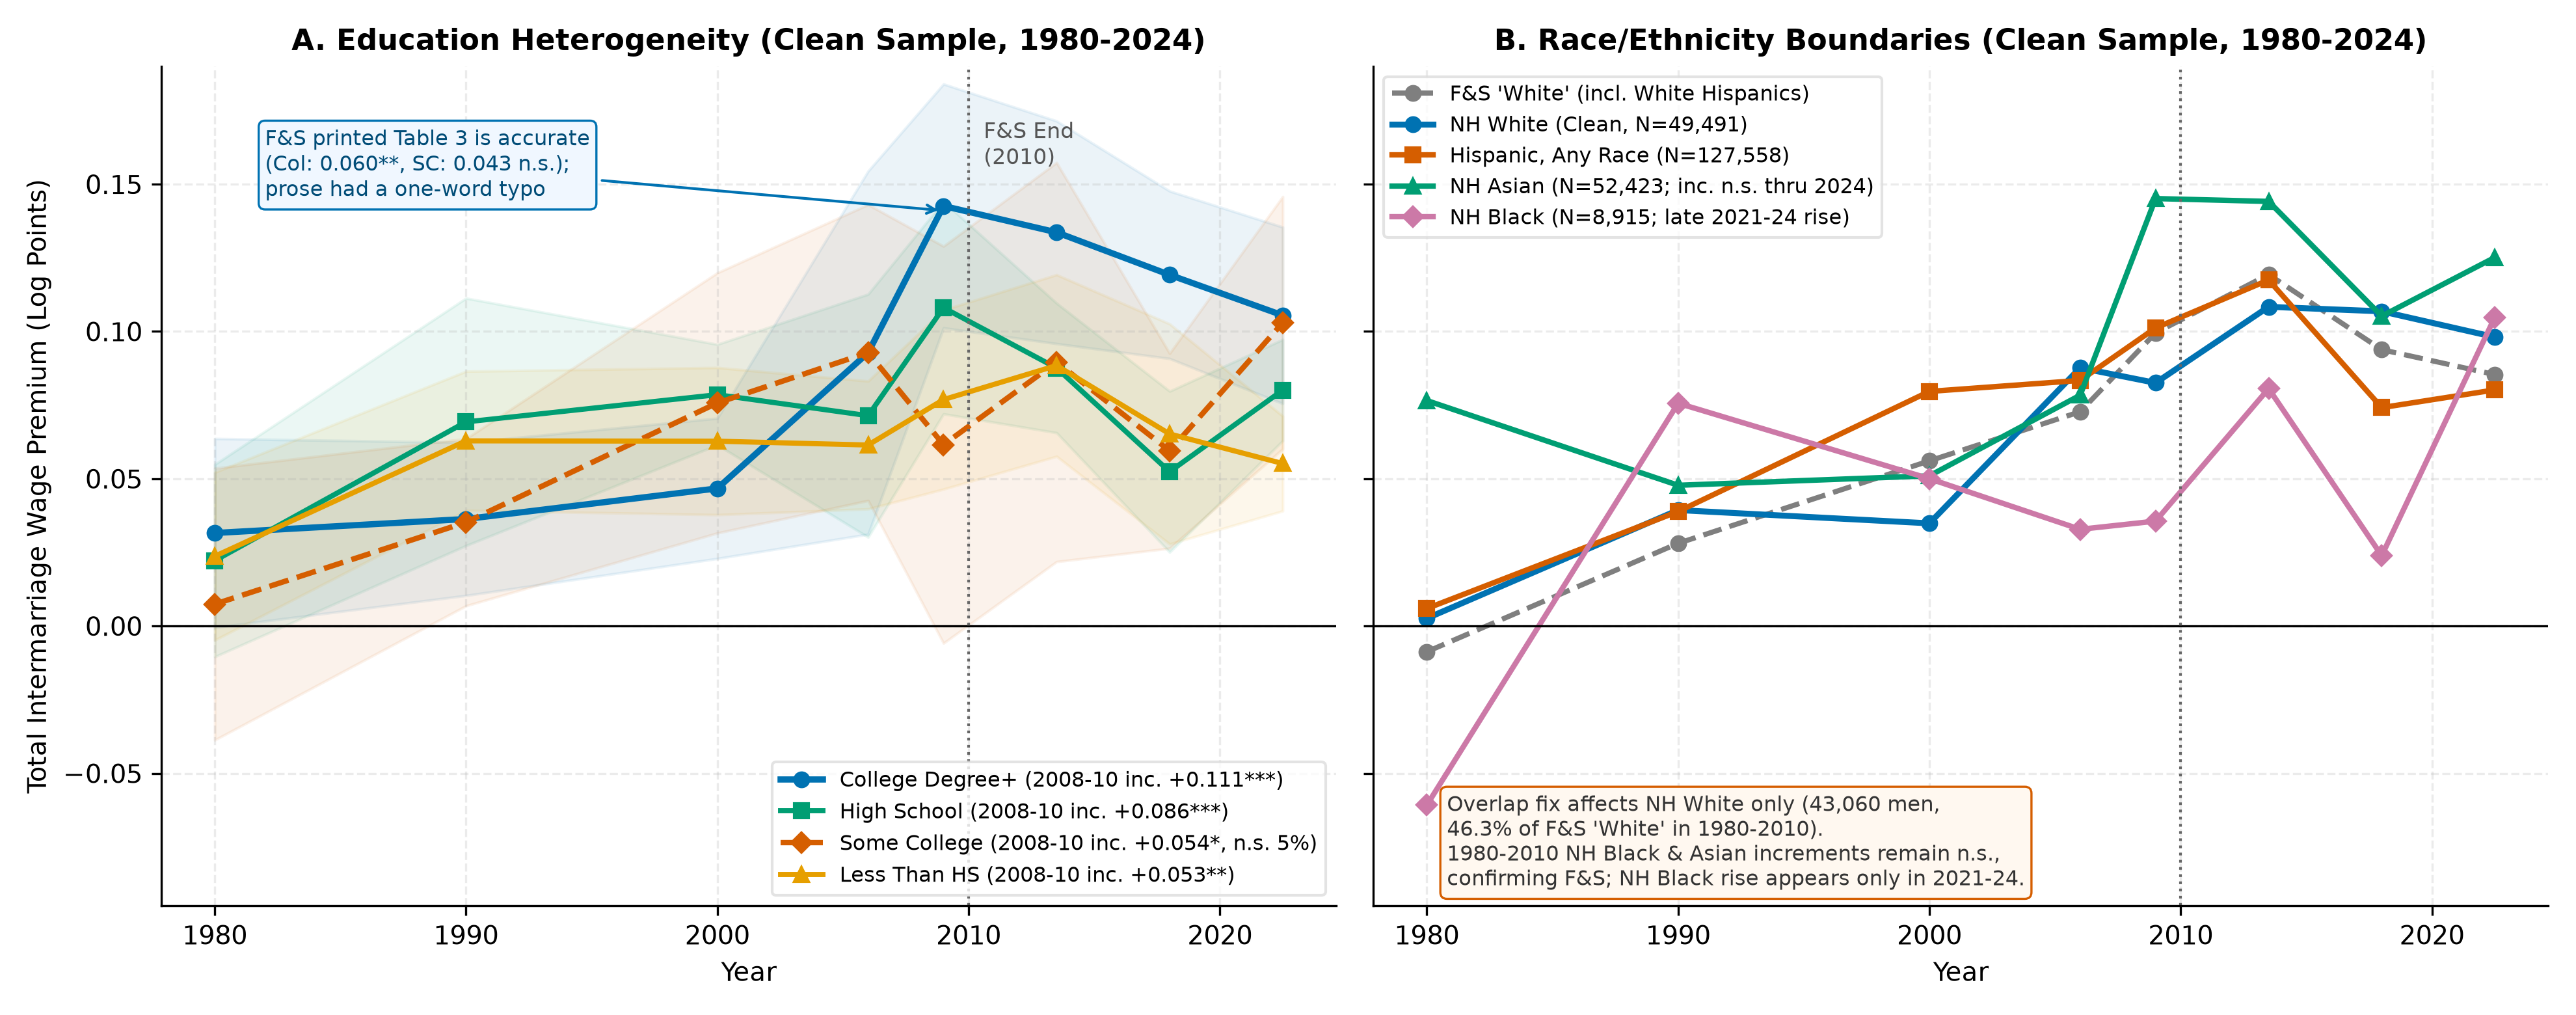
\includegraphics[width=0.92\linewidth,height=0.33\textheight,keepaspectratio]{figures/fig1_forensic_table3_table4.png}
\caption{Conditional Intermarriage Differentials by Education and Race/Ethnicity, 1980--2024. \normalfont Panel~A plots clean true-immigrant male differentials by education ($N = 243{,}707$); college graduates recorded the steepest pre-2010 rise before easing after 2010. Panel~B shows that removing White-identifying Hispanics affects only Non-Hispanic White men, while 1980--2010 Non-Hispanic Black and Asian increments remain statistically insignificant.}
\label{fig:forensic}
\end{figure}

\section{Gelbach (2016) Decomposition and Competing Occupational Task Mediators}
To apportion changes in the conditional intermarriage differential across correlated covariates without arbitrary sequential ordering, we apply Gelbach's (2016) exact order-invariant decomposition. Let $\Delta\hat{\beta}^{\text{base}}$ denote a period-to-period change in the conditional differential from a base model controlling for age, age squared, children, years in the United States, a quadratic in the full-population enclave share, arrival-age bins, origin-by-period fixed effects, and MSA-by-period fixed effects, and let $\Delta\hat{\beta}^{\text{full}}$ denote the same change after adding all $K$ covariate blocks simultaneously. By Frisch--Waugh--Lovell,
\begin{equation}
\Delta\hat{\beta}^{\text{base}} - \Delta\hat{\beta}^{\text{full}} \equiv \sum_{k=1}^{K} \hat{\delta}_k, \qquad \hat{\delta}_k = c'\hat{\Gamma}_k \hat{\beta}_{2,k}^{\text{full}},
\end{equation}
which holds to $<10^{-13}$ in every sample, with two-way cluster-robust standard errors computed via stacked influence functions (Gelbach, 2016, Eq.~11). As with the baseline regressions, Gelbach provides an exact conditional accounting of OLS associations rather than causal mediation, and occupation is a post-marriage mediator.

\begin{table}[t!]\centering
\caption{Gelbach (2016) Decomposition and Competing Occupational Task Mediators (Clean True-Immigrant Men)}
\label{tab:gelbach_decomp}
\scriptsize
\renewcommand{\arraystretch}{0.95}
\setlength{\tabcolsep}{3.0pt}
\resizebox{\linewidth}{!}{%
\begin{tabular}{lcccccc}
\toprule
 & \multicolumn{2}{c}{1980--2024 (No Tasks)} & \multicolumn{4}{c}{2000--2024 Net Rise (2000$\to$2021--24, Common Task Sample)} \\
\cmidrule(lr){2-3} \cmidrule(lr){4-7}
Mediator Block & 1980$\to$12--15 & 12--15$\to$21--24 & Social+Eng & O*NET Math & ALM Tasks & Horse Race \\
\midrule
\textbf{Base Trend ($\Delta \hat{\beta}^{\text{base}}$)} & 0.134*** & -0.017* & 0.050** & 0.050** & 0.050** & 0.050** \\
 & (0.019) & (0.010) & (0.024) & (0.024) & (0.024) & (0.024) \\
Own Education $\times$ Period & 0.036*** & 0.001 & 0.012** & 0.012*** & 0.014*** & 0.010** \\
 & (0.009) & (0.006) & (0.005) & (0.004) & (0.005) & (0.004) \\
\textit{\quad Share of Base} & [26.8\%] & [-7.2\%] & [23.1\%] & [22.8\%] & [27.8\%] & [18.9\%] \\
English Fluency $\times$ Period & 0.002* & -0.001 & -0.002 & -0.002 & -0.001 & -0.002 \\
 & (0.001) & (0.003) & (0.003) & (0.003) & (0.003) & (0.003) \\
Naturalized Citizen $\times$ Period & 0.001 & 0.001 & 0.000 & 0.000 & 0.000 & 0.000 \\
 & (0.002) & (0.001) & (0.001) & (0.001) & (0.001) & (0.001) \\
Spouse Assortative Mating & 0.017*** & -0.004 & 0.005 & 0.005 & 0.006 & 0.005 \\
 & (0.004) & (0.004) & (0.003) & (0.003) & (0.004) & (0.003) \\
\textit{\quad Share of Base} & [12.3\%] & [23.9\%] & [10.5\%] & [10.1\%] & [11.3\%] & [9.3\%] \\
O*NET Social \& English $\times$ Period & --- & --- & 0.029*** & --- & --- & 0.007** \\
 &  &  & (0.005) &  &  & (0.003) \\
\textit{\quad Share of Base} &  &  & [57.7\%] &  &  & [14.2\%] \\
O*NET Math/Analytical $\times$ Period & --- & --- & --- & 0.027*** & --- & 0.023*** \\
 &  &  &  & (0.006) &  & (0.005) \\
\textit{\quad Share of Base} &  &  &  & [54.4\%] &  & [45.4\%] \\
ALM Abstract \& RTI $\times$ Period & --- & --- & --- & --- & 0.023*** & --- \\
 &  &  &  &  & (0.003) &  \\
\textit{\quad Share of Base} &  &  &  &  & [45.8\%] &  \\
\midrule
\textbf{Total Explained ($\sum_k \hat{\delta}_k$)} & 0.056*** & -0.003 & 0.045*** & 0.043*** & 0.042*** & 0.043*** \\
 & (0.011) & (0.007) & (0.013) & (0.013) & (0.012) & (0.013) \\
\textit{\quad Share of Base} & [41.6\%] & [18.4\%] & [88.7\%] & [84.9\%] & [83.0\%] & [85.2\%] \\
\textbf{Residual / Unexplained ($\Delta \hat{\beta}^{\text{full}}$)} & 0.078*** & -0.014 & 0.006 & 0.008 & 0.009 & 0.007 \\
 & (0.014) & (0.009) & (0.013) & (0.012) & (0.013) & (0.012) \\
\textit{\quad Share of Base} & [58.4\%] & [81.6\%] & [11.3\%] & [15.1\%] & [17.0\%] & [14.8\%] \\
\midrule
Observations & 243,707 & 243,707 & 188,455 & 188,455 & 188,455 & 188,455 \\
Full-Model $R^2$ & 0.404 & 0.404 & 0.425 & 0.440 & 0.423 & 0.441 \\
\bottomrule
\end{tabular}%
}
\begin{minipage}{0.98\textwidth}\vspace{2pt}\scriptsize
\textit{Notes:} Exact Gelbach (2016) order-invariant decomposition on clean true-immigrant men (\texttt{CITIZEN} $\in \{2,3\}$; $\sum_k \hat{\delta}_k \equiv \Delta\hat{\beta}^{\text{base}} - \Delta\hat{\beta}^{\text{full}}$ to $<10^{-13}$). Base controls: age, age$^2$, children, years in U.S., enclave share quadratic, arrival-age bins, Origin$\times$Period FEs, and MSA$\times$Period FEs. Two-way clustered SEs (stacked influence functions) in parentheses; shares in brackets. In direct 2000--2024 regressions conditioning on own education (base 2000$\to$2021--24 rise $+0.025$), Social+English absorbs 84.2\%, O*NET Math absorbs 73.5\%, ALM Abstract+RTI absorbs 68.6\%, and in the joint horse race the 2021--24 interactions are Social $=-0.058^{***}$ (0.011), English $=+0.072^{***}$ (0.018), and Math $=+0.044^{***}$ (0.010). Significance: $^{*} p<0.10$, $^{**} p<0.05$, $^{***} p<0.01$.
\end{minipage}
\end{table}

Table~\ref{tab:gelbach_decomp} and Figure~\ref{fig:gelbach} report the decomposition over 1980--2024 (without task indices) and 2000--2024 (with competing occupational task indices on the identical common task sample of $188{,}455$ men). Without task controls over 1980--2015 ($N = 243{,}707$), men's baseline conditional differential rises by $+0.134^{***}$ (SE $0.019$). Time-varying returns to own education account for $+0.036^{***}$ ($26.8$ percent), and spousal assortative mating---comprising spouse education, employment, and log earnings (Greenwood et al., 2014)---accounts for $+0.017^{***}$ ($12.3$ percent). By contrast, English fluency ($+0.002^{*}$, $1.6$ percent, $p = 0.098$) and cleanly defined naturalized citizenship ($+0.001$, $0.9$ percent, $p = 0.48$) contribute negligibly, indicating that marriage-induced naturalization (cf.\ Chi and Drewianka, 2014) is not a primary driver of the long-run climb. Together, these four blocks account for $41.6$ percent of the rise, leaving $58.4$ percent ($+0.078^{***}$) unexplained in the absence of occupational controls.

Adding competing occupational task indices over 2000--2024 ($N = 188{,}455$; baseline net rise $+0.050^{**}$, SE $0.024$) substantially reframes the mechanism. Entered alone, O*NET Social and English Communication tasks absorb $+0.029^{***}$ ($57.7$ percent), raising the total explained share to $88.7$ percent and leaving an insignificant residual ($+0.006$, $p = 0.66$). Competing cognitive task blocks perform nearly as well: O*NET Math/Analytical alone absorbs $+0.027^{***}$ ($54.4$ percent; total explained $84.9$ percent), and ALM Abstract and RTI tasks absorb $+0.023^{***}$ ($45.8$ percent; total explained $83.0$ percent). When Social, English, and Math tasks enter simultaneously in a joint horse race (Column~6), O*NET Math absorbs $+0.023^{***}$ ($45.4$ percent), whereas O*NET Social and English drop to $+0.007^{**}$ ($14.2$ percent). Direct 2000--2024 wage regressions that already condition on own education (baseline rise $+0.025$) show the same pattern: Social and English tasks absorb $84.2$ percent, O*NET Math absorbs $73.5$ percent, and ALM Abstract and RTI absorb $68.6$ percent; in the joint regression, the 2021--2024 interaction on O*NET Social turns negative ($-0.058^{***}$, SE $0.011$), whereas O*NET English ($+0.072^{***}$, SE $0.018$) and O*NET Math ($+0.044^{***}$, SE $0.010$) remain positive. Among women ($N = 114{,}501$), O*NET Math ($47.0$ percent) likewise explains more of the 2000--2024 rise ($+0.058^{***}$) than O*NET Social and English ($33.4$ percent). The data therefore cannot isolate face-to-face social skills as a unique channel; rather, broad occupational sorting into higher-paying cognitive, analytical, and English-intensive jobs accounts for the bulk of the post-2000 conditional rise.

Decomposing the 2012--2015 to 2021--2024 window further shows that post-2015 changes occurred within rather than across occupations. Over this interval, men's baseline differential shifts by $-0.029^{**}$ in the 2000--2024 task sample ($-0.017^{*}$ in 1980--2024). Because occupational task sorting actually widened over the same period ($+0.012^{***}$), $85.9$ percent ($-0.025^{**}$) of the point-estimate change after 2015 took place \emph{within} occupations rather than through occupational downgrading.

\begin{figure}[htb]\centering
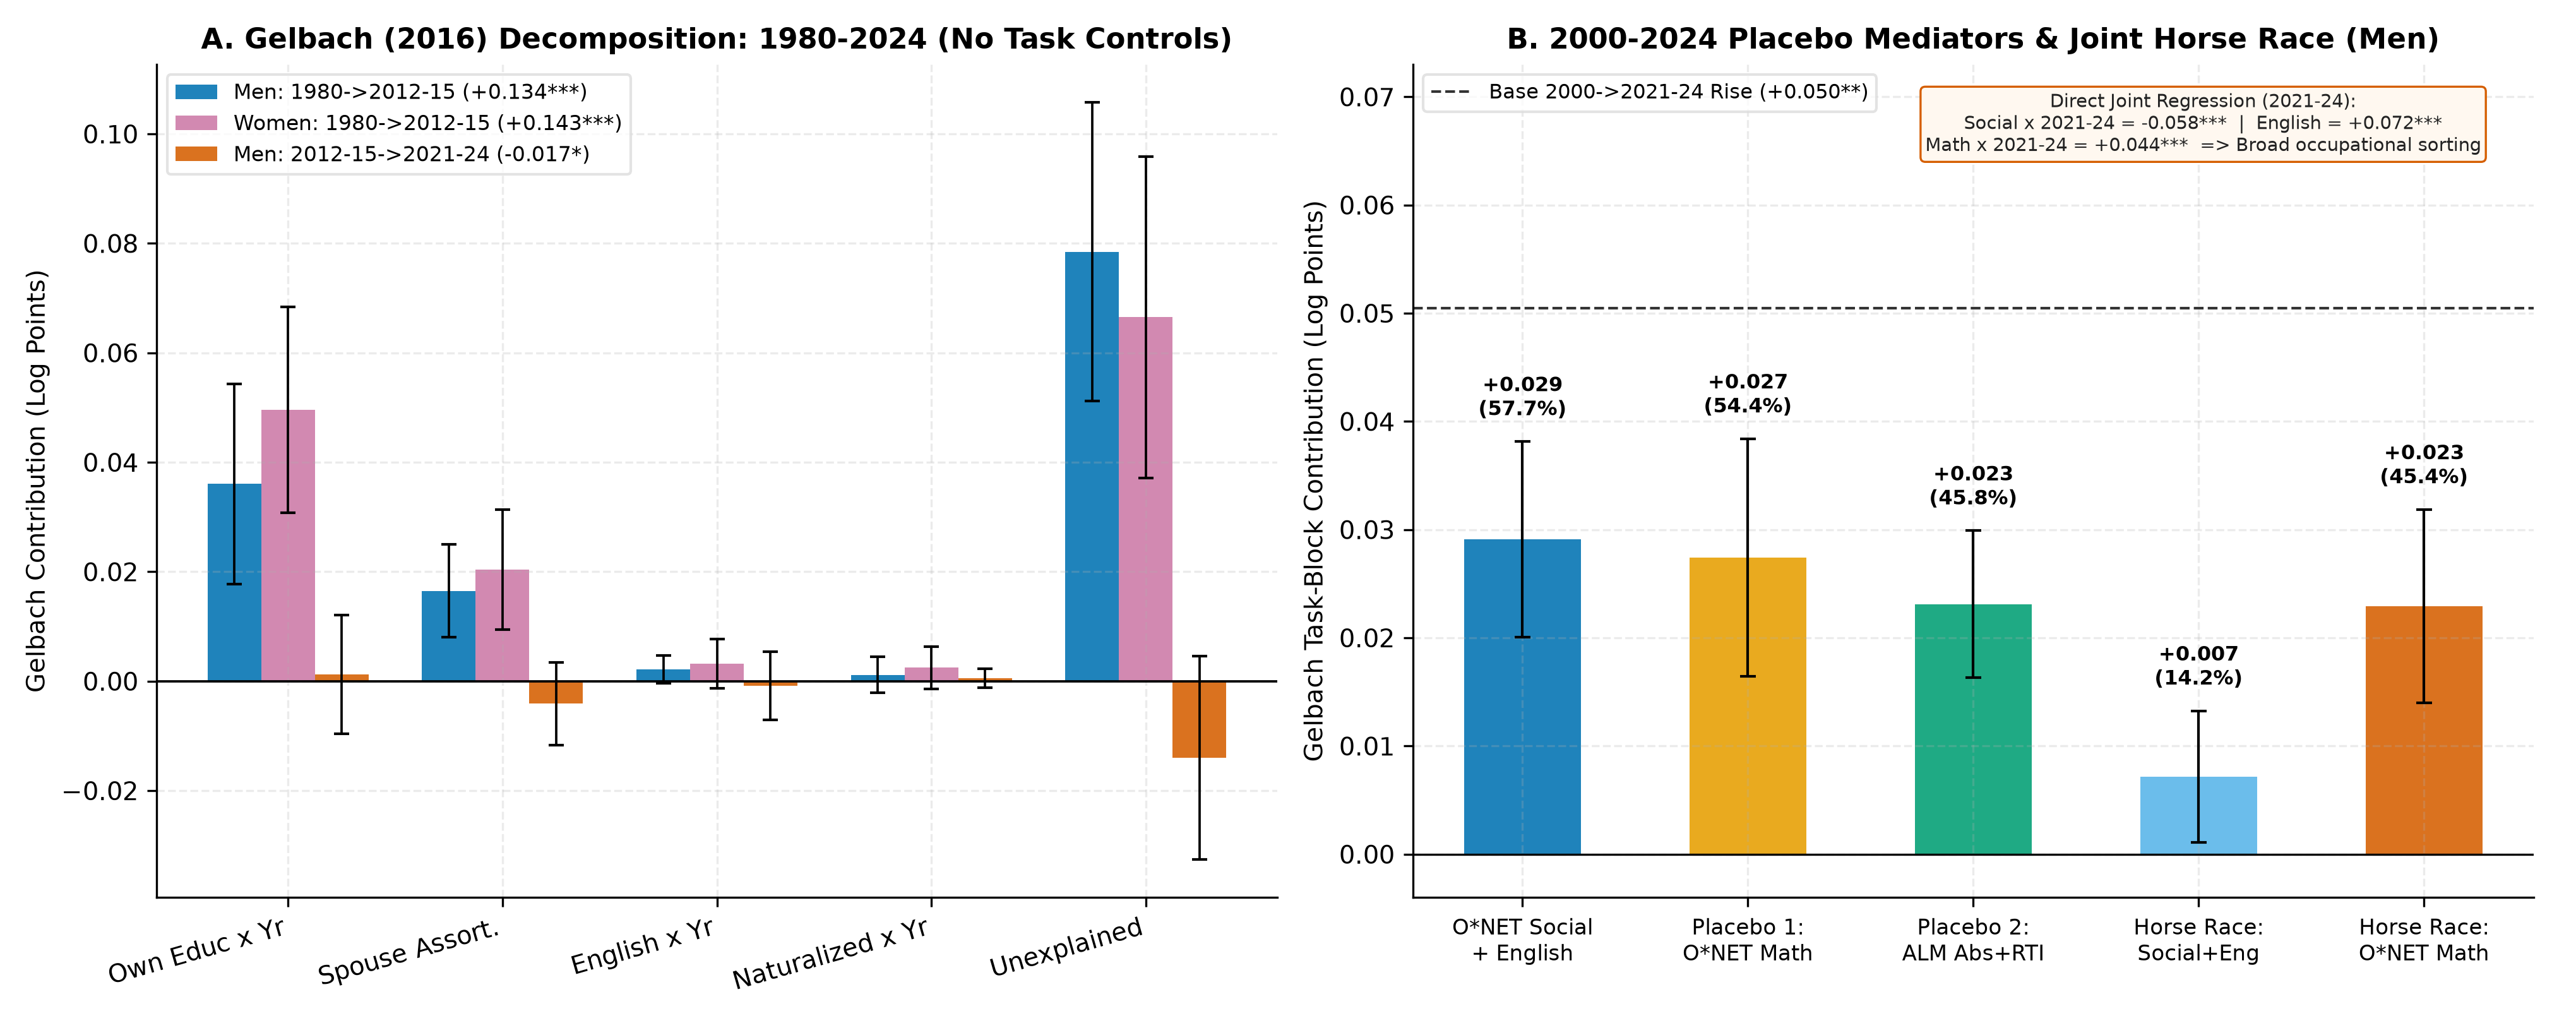
\includegraphics[width=0.92\linewidth,height=0.33\textheight,keepaspectratio]{figures/fig2_gelbach_decomposition.png}
\caption{Gelbach (2016) Decompositions and Competing Occupational Task Mediators, 1980--2024. \normalfont Panel~A reports 1980--2024 Gelbach decompositions without task controls. Panel~B compares task-block contributions across O*NET Social+English, O*NET Math, ALM Abstract+RTI, and a joint horse race on the identical 2000--2024 male sample ($N = 188{,}455$); in the direct joint regression, Social$\times$2021--24 turns negative ($-0.058^{***}$) alongside positive Math ($+0.044^{***}$) and English ($+0.072^{***}$) interactions.}
\label{fig:gelbach}
\end{figure}

\section{Arrival-Age Cohorts and Co-Ethnic Native Spouses}
To probe whether the intermarriage differential reflects English acquisition or broader social networks and selective matching, we apply Bleakley and Chin's (2004, 2010) critical-period arrival-age comparison. We partition the clean male sample into preschool arrivals (ages 0--5; $N = 54{,}416$; $94.8$ percent English-fluent, $86.5$ percent speaking English very well), middle-childhood arrivals (ages 6--11; $N = 61{,}501$; $93.2$ percent fluent), and adolescent arrivals (ages 12--17; $N = 127{,}002$; $80.4$ percent fluent, $52.1$ percent speaking very well).

\begin{table}[t!]\centering
\caption{Arrival-Age Mechanism Test (Ages 0--5 vs.\ 6--11 vs.\ 12--17): Wages, Co-Ethnicity, and Occupational Sorting}
\label{tab:arrival_age}
\scriptsize
\renewcommand{\arraystretch}{0.96}
\setlength{\tabcolsep}{4.5pt}
\resizebox{\linewidth}{!}{%
\begin{tabular}{lccc}
\toprule
 & Ages 0--5 & Ages 6--11 & Ages 12--17 \\
 & (Preschool / Native-Like) & (Middle Childhood) & (Adolescent Arrival) \\
\midrule
\multicolumn{4}{l}{\textbf{Panel A: Weighted Sample Characteristics (Clean True-Immigrant Men, 1980--2024)}} \\
Intermarriage Rate (\%) & 55.2\% & 38.4\% & 21.4\% \\
English Fluent / Very Well (\%) & 94.8\% / 86.5\% & 93.2\% / 78.6\% & 80.4\% / 52.1\% \\
College Degree+ / Naturalized (\%) & 36.9\% / 77.3\% & 33.5\% / 73.9\% & 21.3\% / 57.1\% \\
\midrule
\multicolumn{4}{l}{\textbf{Panel B: 1980--2024 Intermarriage Wage Premium (Log Hourly Wage)}} \\
Intermarriage (1980 Base) & 0.017 & 0.026 & -0.002 \\
 & (0.028) & (0.019) & (0.015) \\
Intermarriage $\times$ 2012--2015 ($\Delta$, Peak) & 0.096** & 0.079** & 0.118*** \\
 & (0.037) & (0.036) & (0.023) \\
Intermarriage $\times$ 2021--2024 ($\Delta$) & 0.057** & 0.092*** & 0.086*** \\
 & (0.028) & (0.023) & (0.021) \\
2021--2024 Total: Non-Co-Ethnic Native & 0.072*** & 0.136*** & 0.122*** \\
 & (0.019) & (0.019) & (0.020) \\
2021--2024 Total: Co-Ethnic U.S.-Born & 0.074*** & 0.098*** & 0.056*** \\
 & (0.015) & (0.016) & (0.014) \\
\midrule
\multicolumn{4}{l}{\textbf{Panel C: 2000--2024 O*NET Occupational Sorting (SD) \& Wage Controls}} \\
O*NET Social Skill Gap (2021--24 Total, SD) & 0.101*** & 0.082*** & 0.091*** \\
 & (0.020) & (0.025) & (0.011) \\
O*NET English Comm.\ Gap (2021--24 Total, SD) & 0.102*** & 0.081*** & 0.099*** \\
 & (0.014) & (0.020) & (0.009) \\
O*NET Math/Analytical Gap (2021--24 Total, SD) & 0.084*** & 0.070*** & 0.073*** \\
 & (0.017) & (0.020) & (0.009) \\
2021--24 Wage Premium: Pre-Task Controls & 0.073*** & 0.115*** & 0.085*** \\
 & (0.013) & (0.012) & (0.014) \\
2021--24 Wage Premium: Post-All O*NET Tasks & 0.047*** & 0.094*** & 0.066*** \\
 & (0.015) & (0.009) & (0.015) \\
\midrule
Observations (1980--2024) & 54,416 & 61,501 & 127,002 \\
\bottomrule
\end{tabular}%
}
\begin{minipage}{0.95\textwidth}\vspace{2pt}\scriptsize
\textit{Notes:} Separate regressions by age at arrival for clean true-immigrant married FTFY men (\texttt{CITIZEN} $\in \{2,3\}$). All regressions include individual controls, enclave share quadratic, Origin$\times$Period FEs, and MSA$\times$Period FEs. Two-way clustered SEs (origin country and MSA) in parentheses. Significance: $^{*} p<0.10$, $^{**} p<0.05$, $^{***} p<0.01$.
\end{minipage}
\end{table}

Table~\ref{tab:arrival_age} and Figure~\ref{fig:arrival} indicate that both language barriers and non-linguistic matching or network channels operate. Preschool arrivals (ages 0--5) already possess native-like English before adulthood, yet their conditional wage differential still rose by $+0.096^{**}$ from 1980 ($0.017$) to 2012--2015 ($0.113^{***}$) before settling at $0.073^{***}$ in 2021--2024. Consistent with broad occupational sorting, intermarried preschool arrivals widened their occupational sorting between 2000 and 2021--2024 across \emph{all three} task indices: O*NET Social, O*NET English Communication, and O*NET Math/Analytical. Adolescent arrivals (ages 12--17) experienced the steepest 1980--2015 wage climb ($+0.118^{***}$, from $-0.002$ to $0.116^{***}$, standing at $0.084^{***}$ in 2021--2024), while middle-childhood arrivals (ages 6--11) rose steadily to $0.117^{***}$ in 2021--2024.

Splitting U.S.-born spouses by co-ethnicity (Duncan and Trejo, 2011) reinforces this interpretation. Across every arrival cohort, marrying either a non-co-ethnic or a co-ethnic U.S.-born spouse is associated with statistically significant 2021--2024 wage differentials: $0.122^{***}$ (non-co-ethnic) and $0.056^{***}$ (co-ethnic) for adolescent arrivals, $0.136^{***}$ and $0.098^{***}$ for middle-childhood arrivals, and $0.072^{***}$ and $0.074^{***}$ for preschool arrivals. Local networks, institutional familiarity, and selective partner matching thus appear relevant both across and within ethnic boundaries.

\begin{figure}[htb]\centering
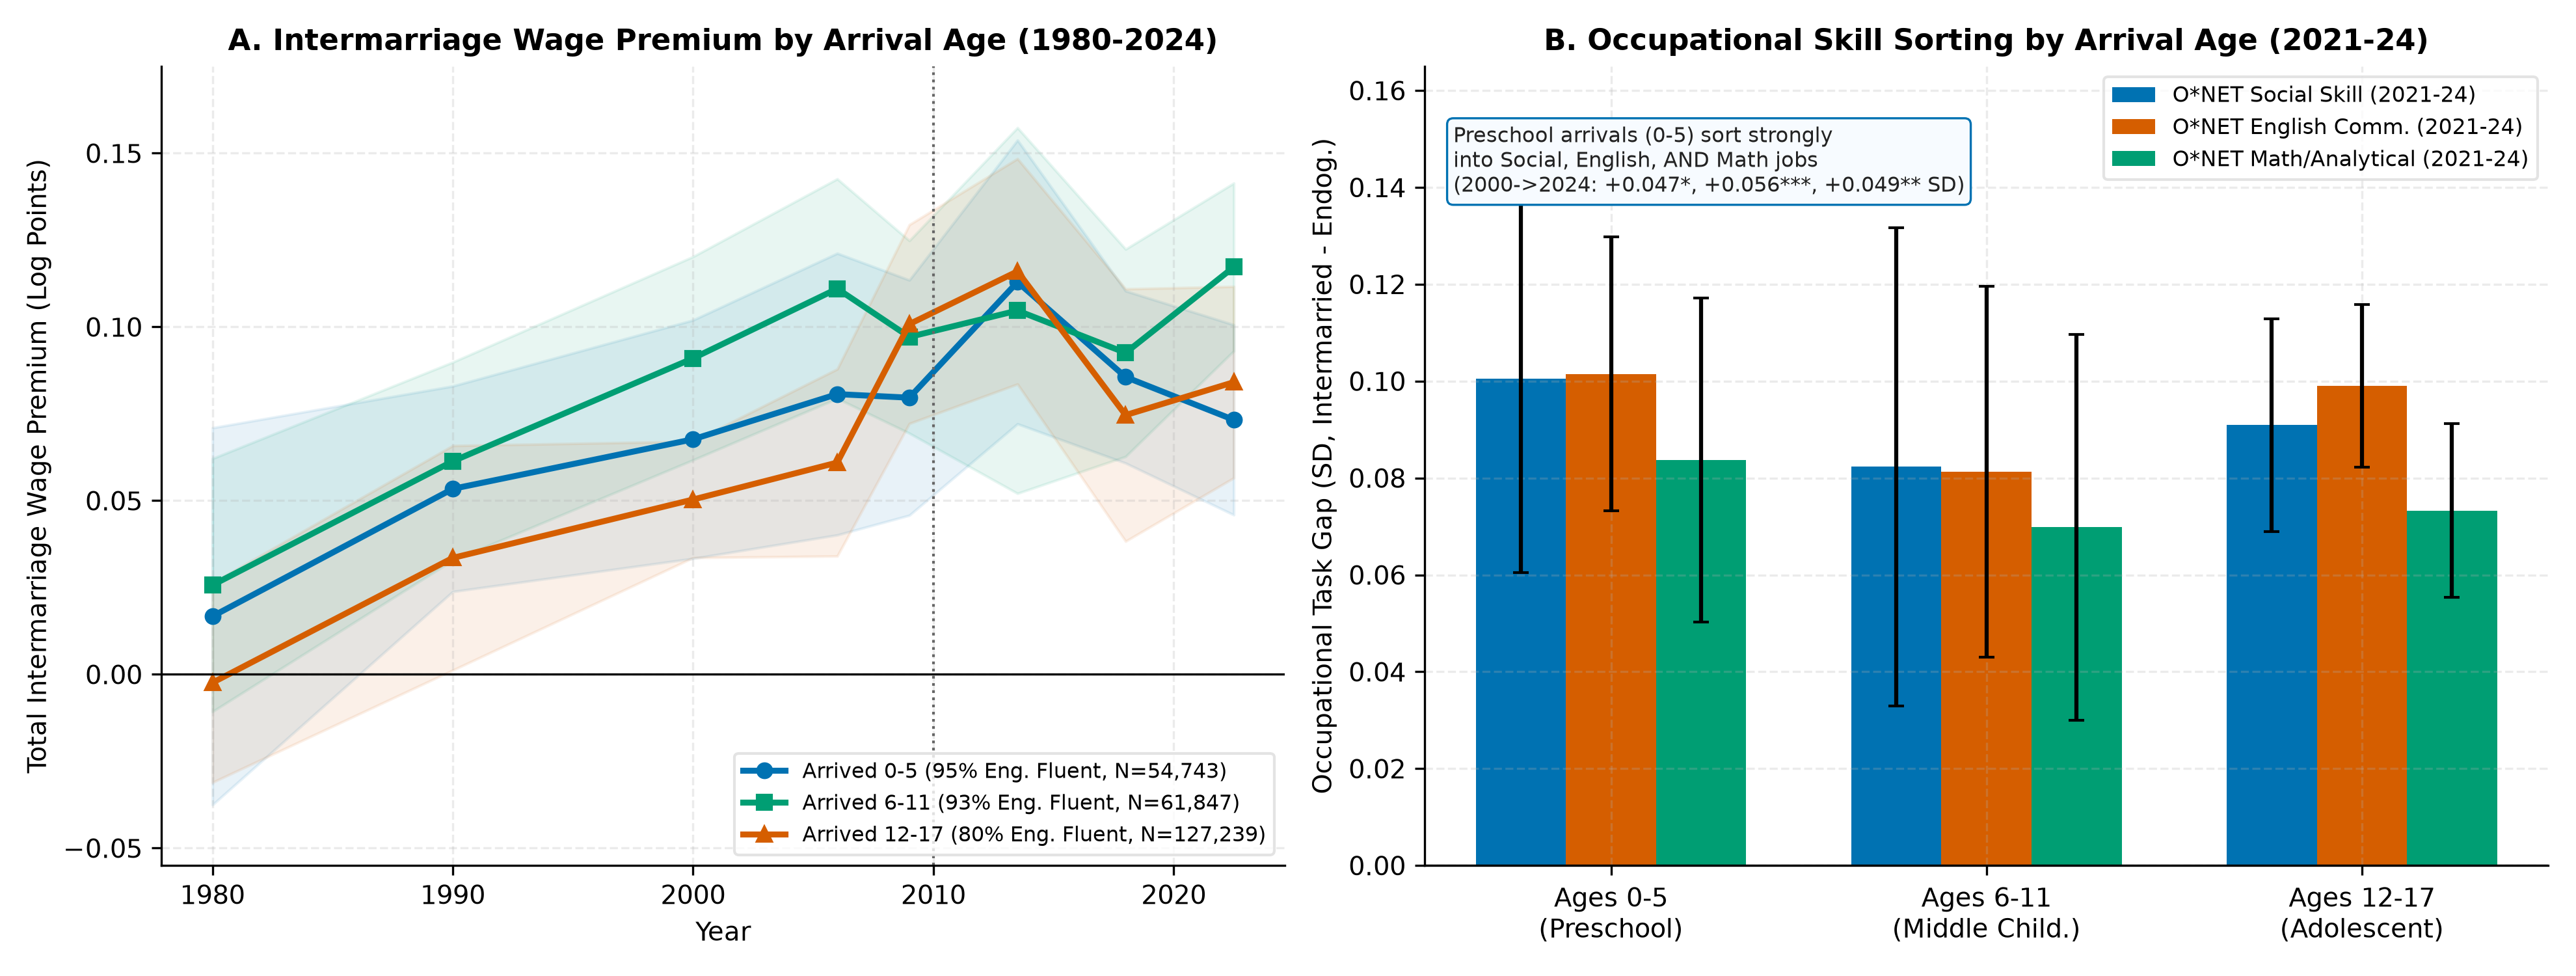
\includegraphics[width=0.92\linewidth,height=0.33\textheight,keepaspectratio]{figures/fig3_arrival_age_mechanism.png}
\caption{Conditional Wage Differentials and Occupational Task Sorting by Age at Arrival, 1980--2024. \normalfont Panel~A tracks 1980--2024 conditional wage differentials by arrival-age cohort on the clean true-immigrant male sample. Panel~B displays 2021--2024 occupational task gaps (in standard deviations) across O*NET Social, English Communication, and Math/Analytical indices.}
\label{fig:arrival}
\end{figure}

\section{Gender Convergence, Cohabitation, and Selection Correction}
Extending the clean true-immigrant framework to $141{,}327$ married FTFY 1.5-generation women reveals gradual post-2015 convergence with men. Whereas men's baseline differential reached $0.115^{***}$ in 2012--2015 and stood at $0.094^{***}$ in 2021--2024 (direct change $-0.021$, $p = 0.084$), women's aggregate differential climbed from $-0.018^{*}$ in 1980 to $0.088^{***}$ in 2008--2010, $0.091^{***}$ in 2012--2015, and $0.101^{***}$ in 2021--2024 (direct change $+0.010$, 95 percent CI $[-0.025, +0.046]$, $p = 0.556$). Table~\ref{tab:gender_ipw} and Figure~\ref{fig:gender} evaluate education heterogeneity, household specialization, cohabitation, and sample selection.

\begin{table}[t!]\centering
\caption{Gender Convergence, Household Specialization, Cohabitation Pooling, IPW Selection Correction, and Oster (2019) Bounds}
\label{tab:gender_ipw}
\scriptsize
\renewcommand{\arraystretch}{0.95}
\setlength{\tabcolsep}{3.5pt}
\resizebox{\linewidth}{!}{%
\begin{tabular}{lcccccc}
\toprule
 & \multicolumn{3}{c}{1.5-Gen Men (Clean)} & \multicolumn{3}{c}{1.5-Gen Women (Clean)} \\
\cmidrule(lr){2-4} \cmidrule(lr){5-7}
Specification / Subsample (Total Premium) & 2008--10 & 2012--15 & 2021--24 & 2008--10 & 2012--15 & 2021--24 \\
\midrule
\multicolumn{7}{l}{\textbf{Panel A: Education Heterogeneity (College+ vs.\ Non-College)}} \\
College Degree+ & 0.143*** & 0.134*** & 0.105*** & 0.087*** & 0.082*** & 0.111*** \\
 & (0.021) & (0.019) & (0.015) & (0.021) & (0.019) & (0.015) \\
Non-College ($<$ BA) & 0.088*** & 0.098*** & 0.084*** & 0.083*** & 0.083*** & 0.077*** \\
 & (0.010) & (0.010) & (0.010) & (0.013) & (0.013) & (0.014) \\
\midrule
\multicolumn{7}{l}{\textbf{Panel B: Household Specialization Controls (Spouse Hours, Employment, Children $\times$ Period)}} \\
Baseline (Origin$\times$Yr + MSA$\times$Yr FEs) & 0.101*** & 0.115*** & 0.094*** & 0.088*** & 0.091*** & 0.101*** \\
 & (0.010) & (0.011) & (0.011) & (0.014) & (0.011) & (0.016) \\
+ Spouse Hours, Emp., Children $\times$ Yr & 0.109*** & 0.121*** & 0.099*** & 0.087*** & 0.091*** & 0.100*** \\
 & (0.010) & (0.014) & (0.012) & (0.014) & (0.011) & (0.017) \\
+ Spouse Educ. \& Earnings $\times$ Yr & 0.090*** & 0.091*** & 0.077*** & 0.070*** & 0.065*** & 0.083*** \\
 & (0.010) & (0.014) & (0.012) & (0.015) & (0.011) & (0.018) \\
\midrule
\multicolumn{7}{l}{\textbf{Panel C: Cohabitation Pooling (1990--2024) \& IPW Selection-into-(Marriage$\times$FTFY) Correction}} \\
Married Only (1990--2024) & 0.099*** & 0.113*** & 0.093*** & 0.087*** & 0.090*** & 0.100*** \\
 & (0.010) & (0.011) & (0.011) & (0.013) & (0.011) & (0.016) \\
Pooled Married + Cohabiting (1990--2024) & 0.096*** & 0.109*** & 0.086*** & 0.091*** & 0.090*** & 0.090*** \\
 & (0.009) & (0.010) & (0.008) & (0.014) & (0.011) & (0.014) \\
IPW Selection-Corrected (1980--2024) & 0.083*** & 0.100*** & 0.088*** & 0.081*** & 0.092*** & 0.080*** \\
 & (0.009) & (0.007) & (0.009) & (0.011) & (0.010) & (0.014) \\
IPW + Full Mechanism Controls & 0.075*** & 0.078*** & 0.074*** & 0.059*** & 0.066*** & 0.071*** \\
 & (0.011) & (0.012) & (0.010) & (0.011) & (0.013) & (0.015) \\
\midrule
\multicolumn{7}{l}{\textbf{Panel D: Oster (2019) Coefficient-Stability Bounds ($\delta$ / $\beta^*(\delta=1)$, $R_{\max}=1.3 R^2$)}} \\
Baseline: $\delta$ / $\beta^*(\delta=1)$ & -47.6 / 0.105 & -7.9 / 0.132 & -3.0 / 0.129 & 4.1 / 0.080 & 4.5 / 0.084 & 9.7 / 0.106 \\
IPW-Corrected: $\delta$ / $\beta^*(\delta=1)$ & -25.5 / 0.089 & -3.9 / 0.129 & -1.9 / 0.138 & 3.8 / 0.079 & 6.7 / 0.100 & $>50$ / 0.106 \\
\bottomrule
\end{tabular}%
}
\begin{minipage}{0.98\textwidth}\vspace{2pt}\scriptsize
\textit{Notes:} Total log hourly wage premiums for clean true-immigrant 1.5-generation workers (\texttt{CITIZEN} $\in \{2,3\}$). IPW weights predict selection into Married$\times$FTFY$\times$Valid-Wage separately by sex and period from the 1.53M true-immigrant 1.5-generation universe (logit AUC = 0.80--0.82 for men, 0.65--0.71 for women), stabilized and trimmed at the 1st/99th percentiles. Negative Oster $\delta$ indicates controls raise the estimated trend relative to the raw gap. Two-way clustered SEs in parentheses. Significance: $^{*} p<0.10$, $^{**} p<0.05$, $^{***} p<0.01$.
\end{minipage}
\end{table}

\subsection{College-Educated Gender Convergence and Household Specialization}
Panel~A of Table~\ref{tab:gender_ipw} and Figure~\ref{fig:gender}A show that college graduates drive this convergence. Among college-educated men ($N = 73{,}284$), the differential peaked in 2008--2010 at $0.143^{***}$ and eased to $0.134^{***}$ in 2012--2015 and $0.105^{***}$ in 2021--2024 (direct 2021--2024 minus 2012--2015 change $-0.028$, $p = 0.280$). Among college-educated women ($N = 53{,}803$), the differential moved in the opposite direction, rising from $0.082^{***}$ in 2012--2015 to $0.111^{***}$ in 2021--2024 (direct change $+0.029$, $p = 0.119$) and reaching parity with college men---consistent with broader gains by college-educated women in high-paying professional and managerial occupations (Cortes, Jaimovich, and Siu, 2023). By contrast, non-college women ($N = 87{,}028$) remained flat from 2008--2010 through 2021--2024 ($0.083^{***}$, $0.083^{***}$, and $0.077^{***}$).

Panel~B tests whether changing household specialization explains the gender pattern by adding spouse usual weekly hours, spouse employment status, and number of children interacted with every period. These controls leave both men's path ($0.115^{***}\to 0.094^{***}$ versus $0.121^{***}\to 0.099^{***}$) and women's path ($0.091^{***}\to 0.101^{***}$ versus $0.091^{***}\to 0.100^{***}$) essentially unchanged. Further adding spouse education and spouse log earnings lowers levels by roughly $1.7$ to $2.9$ log points across 2008--2024 for both sexes without altering the post-2015 convergence.

\subsection{Cohabitation Pooling, Stabilized IPW, and Oster (2019) Bounds}
Because formal marriage rates declined and unmarried cohabitation rose over 1980--2024, Panels~C and~D of Table~\ref{tab:gender_ipw} and Figure~\ref{fig:gender}B assess sensitivity to selection into formal marriage and full-time employment. Pooling $25{,}282$ cohabiting FTFY men ($N = 252{,}698$ total) and $17{,}549$ cohabiting FTFY women ($N = 151{,}701$ total) over 1990--2024 with a cohabitation indicator preserves men's post-2015 trajectory ($0.109^{***}$ in 2012--2015 to $0.086^{***}$ in 2021--2024) while completely flattening women's post-2015 profile ($0.090^{***}$ in 2012--2015 to $0.090^{***}$ in 2021--2024).

To adjust for observable selection out of the $1.53$-million true-immigrant 1.5-generation universe, we estimate period- and sex-specific weighted logistic models predicting inclusion in the married, full-time, valid-wage sample from age, age squared, education, English fluency, naturalized citizenship, children, arrival-age bins, race/ethnicity, and full-population enclave share (AUC $0.80$--$0.82$ for men; $0.65$--$0.71$ for women), trimming stabilized weights at the 1st and 99th percentiles. For men, IPW trims levels by roughly 1 to 1.5 log points and flattens the post-2015 contrast further ($0.100^{***}$ in 2012--2015 to $0.088^{***}$ in 2021--2024; direct change $-0.012$, $p = 0.207$; $0.078^{***}$ to $0.074^{***}$ with full mechanism controls). For women, IPW reverses the small aggregate post-2015 uptick ($0.092^{***}$ in 2012--2015 to $0.080^{***}$ in 2021--2024; direct change $-0.012$, $p = 0.517$), indicating that women's aggregate post-2015 rise reflects both college-female convergence and growing positive selection into formal marriage and full-time work.

Finally, Oster (2019) proportional-selection bounds under $R_{\max} = 1.3 R^2$ (Panel~D) confirm that unobservable selection would have to be substantially stronger than observable selection ($|\delta| \ge 1.9$ for men; $\delta \ge 3.8$ for women) or operate in the opposite direction ($\delta < 0$ for men, where controls raise the estimated trend) to explain away the post-2000 rise. At $\delta = 1$, bias-adjusted bounds remain solidly positive across all post-2000 periods reported in Panel~D ($\beta^{*}(\delta=1) \in [+0.079, +0.138]$ across 2008--2024).

\begin{figure}[htb]\centering
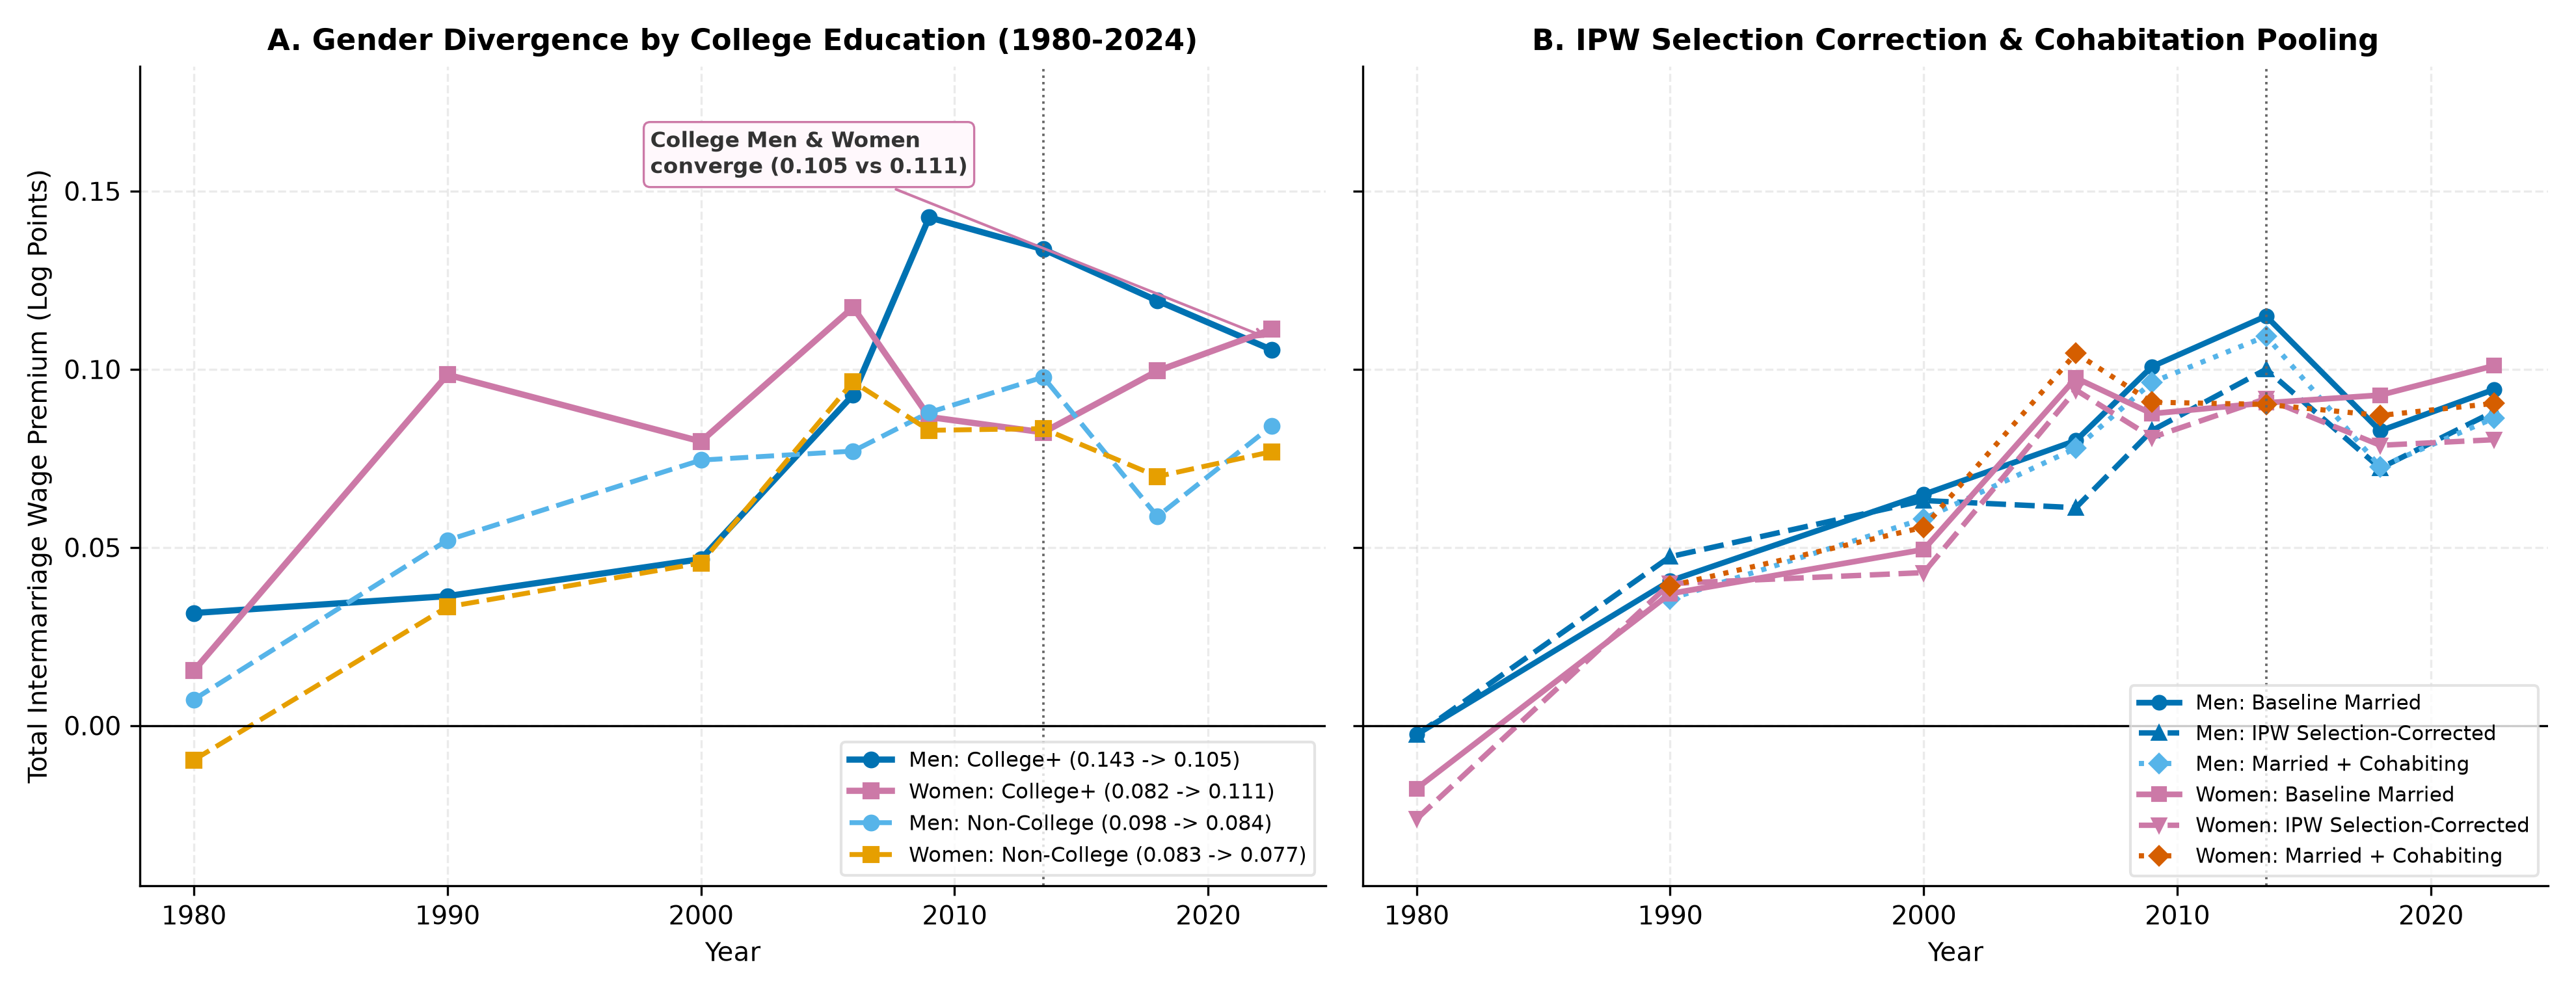
\includegraphics[width=0.92\linewidth,height=0.33\textheight,keepaspectratio]{figures/fig4_gender_divergence_selection.png}
\caption{Gender Convergence, Cohabitation Pooling, and Selection Correction, 1980--2024. \normalfont Panel~A plots clean-sample conditional differentials by sex and college degree. Panel~B compares baseline married estimates against cohabitation-pooled and IPW-reweighted series.}
\label{fig:gender}
\end{figure}

\subsection{Limitations and Scope}
Several scope boundaries govern interpretation. Partner choice is endogenous, so every regression identifies conditional earnings differentials rather than causal treatment effects. Similarly, Gelbach (2016) provides an exact conditional accounting of OLS associations in which occupation is a post-marriage mediator; our competing task tests show that correlated occupation-level indices cannot isolate communication skills from broad sorting across jobs. On selection, IPW adjusts strictly for selection on observables (with lower first-stage AUC for women than for men), and Oster (2019) bounds rely on proportional selection and $R_{\max} = 1.3 R^2$. Finally, O*NET and ALM task scores are time-invariant occupation averages mapped onto 2000--2024 repeated cross-sections rather than longitudinal measures of individual skill acquisition, and our full-population enclave denominators cover working-age residents aged 18--64.

\FloatBarrier
\section{Conclusion}
Replicating Furtado and Song (2015) with full-population working-age metropolitan enclave denominators and extending their analysis by fourteen years through 2024 confirms their central 1980--2010 empirical finding while reframing its post-2010 trajectory and underlying mechanism. Among true foreign-born childhood-arrival men, the conditional intermarriage differential remained substantial after the Great Recession without continuing its earlier climb, reaching its highest point estimate in 2012--2015 ($0.115$ log points) and standing at $0.094$ log points in 2021--2024. The direct latest-minus-peak contrast of $-0.021$ log points (95 percent CI $[-0.044, +0.003]$, $p = 0.084$) offers little evidence of continued growth while falling short of a statistically significant decline at the 5 percent level. The absence of post-2015 growth holds across foreign-born enclave denominators and time-consistent state and metropolitan fixed effects, whereas retaining birthright U.S.\ citizens born abroad sharpens the latest-minus-peak contrast to a statistically significant $-0.025$ log points ($p = 0.017$)---underscoring why isolating true foreign-born immigrants matters for interpreting post-2015 dynamics.

On mechanisms, Gelbach (2016) decompositions augmented with competing occupational task indices indicate that broad sorting across higher-paying analytical and English-intensive occupations, rather than face-to-face social skills uniquely, accounts for the bulk of the post-2000 conditional rise. O*NET Math alone absorbs $54.4$ percent of men's baseline gain (nearly matching O*NET Social and English at $57.7$ percent) and dominates the joint horse race ($45.4$ versus $14.2$ percent), while in direct regressions conditioning on own education the late-period O*NET Social interaction turns negative ($-0.058$, $p < 0.01$) alongside positive English and Math returns; naturalized citizenship accounts for less than 1 percent. Subgroup audits confirm Furtado and Song's 1980--2010 nulls for Non-Hispanic Black and Asian men under metropolitan clustering and origin-country wild cluster bootstrap inference, college-educated immigrant women reach parity with college-educated men by 2021--2024, and the long-run conditional earnings differential persists across cohabitation pooling, stabilized IPW reweighting, and Oster (2019) bounds.

\FloatBarrier
\clearpage
\begin{thebibliography}{99}
\bibitem{autor2013} Autor, D.~H., \& Dorn, D.\ (2013). The growth of low-skill service jobs and the polarization of the US labor market. \textit{American Economic Review}, 103(5), 1553--1597.
\bibitem{bleakley2004} Bleakley, H., \& Chin, A.\ (2004). Language skills and earnings: Evidence from childhood immigrants. \textit{Review of Economics and Statistics}, 86(2), 481--496.
\bibitem{bleakley2010} Bleakley, H., \& Chin, A.\ (2010). Age at arrival, English proficiency, and social assimilation among US immigrants. \textit{American Economic Journal: Applied Economics}, 2(1), 165--192.
\bibitem{cameron2008} Cameron, A.~C., Gelbach, J.~B., \& Miller, D.~L.\ (2008). Bootstrap-based improvements for inference with clustered errors. \textit{Review of Economics and Statistics}, 90(3), 414--427.
\bibitem{cameron2011} Cameron, A.~C., Gelbach, J.~B., \& Miller, D.~L.\ (2011). Robust inference with multiway clustering. \textit{Journal of Business \& Economic Statistics}, 29(2), 238--249.
\bibitem{chi2014} Chi, M., \& Drewianka, S.\ (2014). How much is a green card worth? Evidence from Mexican men who marry women born in the U.S.\ \textit{Labour Economics}, 31, 103--116.
\bibitem{cortes2023} Cortes, G.~M., Jaimovich, N., \& Siu, H.~E.\ (2023). The growing importance of social tasks in high-paying occupations: Implications for sorting. \textit{Journal of Human Resources}, 58(5), 1445--1474.
\bibitem{deming2017} Deming, D.~J.\ (2017). The growing importance of social skills in the labor market. \textit{Quarterly Journal of Economics}, 132(4), 1593--1640.
\bibitem{duncan2011} Duncan, B., \& Trejo, S.~J.\ (2011). Intermarriage and the intergenerational transmission of ethnic identity and human capital for Mexican Americans. \textit{Journal of Labor Economics}, 29(2), 195--227.
\bibitem{furtado2015} Furtado, D., \& Song, T.\ (2015). Intermarriage and socioeconomic integration: Trends in earnings premiums among U.S.\ immigrants who marry natives. \textit{The ANNALS of the American Academy of Political and Social Science}, 662(1), 207--222.
\bibitem{furtado2009} Furtado, D., \& Theodoropoulos, N.\ (2009). I'll marry you if you get me a job: Marital assimilation and immigrant employment rates. \textit{International Journal of Manpower}, 30(1/2), 116--126.
\bibitem{furtado2010} Furtado, D., \& Theodoropoulos, N.\ (2010). Why does intermarriage increase immigrant employment? The role of networks. \textit{B.E.\ Journal of Economic Analysis \& Policy}, 10(1), Article~101.
\bibitem{gelbach2016} Gelbach, J.~B.\ (2016). When do covariates matter? And which ones, and how much? \textit{Journal of Labor Economics}, 34(2), 509--543.
\bibitem{greenwood2014} Greenwood, J., Guner, N., Kocharkov, G., \& Santos, C.\ (2014). Marry your like: Assortative mating and income inequality. \textit{American Economic Review}, 104(5), 348--353.
\bibitem{kantarevic2004} Kantarevic, J.\ (2004). Interethnic marriages and economic assimilation of immigrants. \textit{IZA Discussion Paper} No.~1142.
\bibitem{meng2005} Meng, X., \& Gregory, R.~G.\ (2005). Intermarriage and the economic assimilation of immigrants. \textit{Journal of Labor Economics}, 23(1), 135--174.
\bibitem{onet2026} National Center for O*NET Development (2026). \textit{O*NET 31.0 Database}. U.S.\ Department of Labor, Employment and Training Administration. \url{https://www.onetcenter.org/database.html}
\bibitem{oster2019} Oster, E.\ (2019). Unobservable selection and coefficient stability: Theory and evidence. \textit{Journal of Business \& Economic Statistics}, 37(2), 187--204.
\bibitem{ruggles2026} Ruggles, S., Flood, S., Sobek, M., Backman, D., Chen, A., Cooper, G., Richards, S., Rodgers, R., \& Schouweiler, M.\ (2026). \textit{IPUMS USA: Version 16.0} [dataset]. Minneapolis, MN: IPUMS. \url{https://doi.org/10.18128/D010.V16.0}
\bibitem{song2017} Song, T.\ (2017). \textit{Three Essays on Immigrants' Socio-Economic Integration in the United States}. Ph.D.\ Dissertation, Department of Economics, University of Connecticut.
\bibitem{webb2023} Webb, M.~D.\ (2023). Reworking wild bootstrap-based inference for clustered errors. \textit{Canadian Journal of Economics}, 56(3), 839--858.
\end{thebibliography}

\end{document}
